\section{Frontend Architecture and Implementation}

The presentation layer of the DBaaS platform is engineered to abstract the inherent complexities of multi-tenant database management behind an intuitive, declarative user interface. Rather than exposing users to raw Kubernetes manifests or complex SQL DDL commands, the frontend translates user interactions into deterministic API payloads. The architecture strictly adheres to a unidirectional data flow, ensuring that the UI remains a reactive reflection of the backend's state machine.

\subsection{Architectural Rationale: Flutter for the Web}

To construct a highly responsive, single-codebase application capable of rendering complex data grids and interactive schema diagrams, the presentation layer was implemented using \textbf{Flutter}. While traditional Document Object Model (DOM) based frameworks (e.g., ReactJS, VueJS) are prevalent, Flutter's CanvasKit rendering engine was selected for its ability to bypass DOM manipulation bottlenecks, achieving consistent pixel-perfect rendering across all environments.

Table~\ref{tab:flutter_comparison} summarizes the architectural justifications for selecting Flutter over conventional DOM-based web technologies for this specific DBaaS use case.

\begin{table}[h]
\centering
\caption{Comparison of Flutter Web with Other Web Technologies}
\label{tab:flutter_comparison}
\renewcommand{\arraystretch}{1.3}
\begin{tabular}{|l|c|c|c|c|}
\hline
\textbf{Aspect} & \textbf{Flutter Web} & \textbf{ReactJS} & \textbf{Angular} & \textbf{VueJS} \\
\hline
Single Codebase & \ding{51} & \ding{55} & \ding{55} & \ding{55} \\
\hline
Pixel-perfect UI & \ding{51} & \ding{55} & \ding{55} & \ding{55} \\
\hline
Hot Reload / Fast Development & \ding{51} & \ding{51} & \ding{55} & \ding{51} \\
\hline
Enterprise Ready & \ding{55} & \ding{51} & \ding{51} & \ding{55} \\
\hline
Lightweight & \ding{55} & \ding{55} & \ding{55} & \ding{51} \\
\hline
Large Community Support & \ding{51} & \ding{51} & \ding{51} & \ding{51} \\
\hline
Best for Animations & \ding{51} & \ding{55} & \ding{55} & \ding{55} \\
\hline
Easy to Learn & \ding{55} & \ding{55} & \ding{55} & \ding{51} \\
\hline
\end{tabular}
\end{table}
\newpage
\section{Completed and Under Development Features}

This section highlights the core functional modules of the DBaaS platform that have been successfully implemented and verified.

\subsection{Implemented Features}

% --- 1. Authentication ---
\subsubsection*{Authentication Interface}
A secure entry point featuring dual-mode authentication (Sign In/Sign Up), email validation, and password recovery options.



\begin{figure}[H] % تم التغيير لـ H لتثبيتها تحت الكلام مباشرة
    \centering
    \begin{subfigure}[b]{0.48\textwidth}
        \centering
        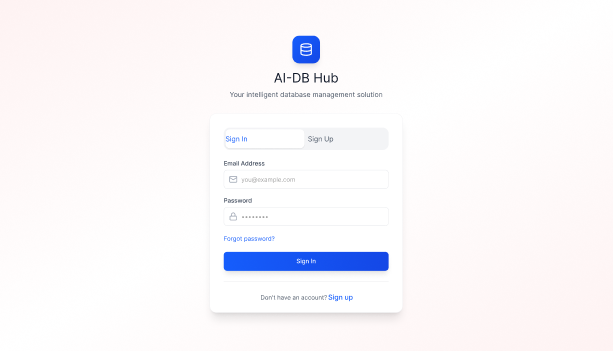
\includegraphics[width=\textwidth]{images/login.png}
        \caption{Login Screen}
    \end{subfigure}
    \hfill
    \begin{subfigure}[b]{0.48\textwidth}
        \centering
        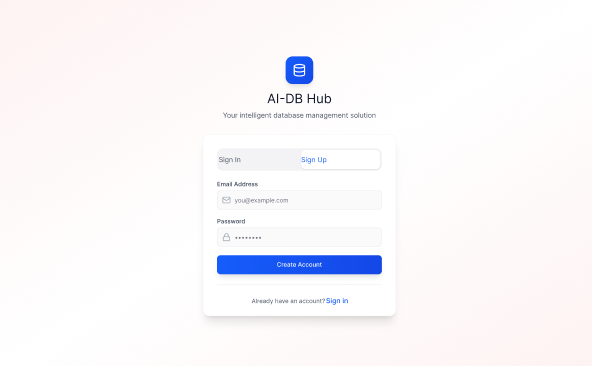
\includegraphics[width=\textwidth]{images/sign up.png}
        \caption{Sign Up Screen}
    \end{subfigure}
    \vspace{5pt}
    \caption{Authentication screens of the DBaaS system.}
\end{figure}

% --- 2. Home Tab & Project Creation ---
\subsubsection*{Project Dashboard \& Provisioning}
The central hub for managing the database lifecycle, including a guided modal for provisioning new cloud instances.

\begin{figure}[H]
    \centering
    \begin{subfigure}[b]{0.48\textwidth}
        \centering
        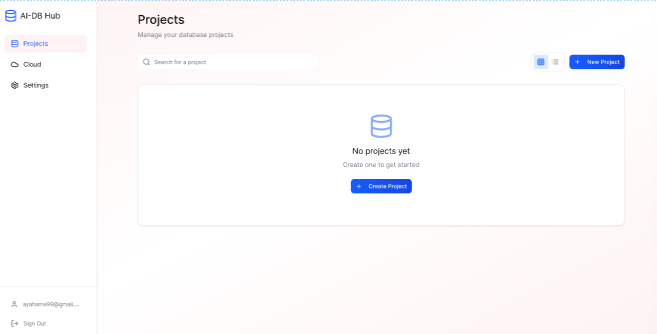
\includegraphics[width=\textwidth]{images/home tab.png}
        \caption{Central Dashboard}
    \end{subfigure}
    \hfill
    \begin{subfigure}[b]{0.48\textwidth}
        \centering
        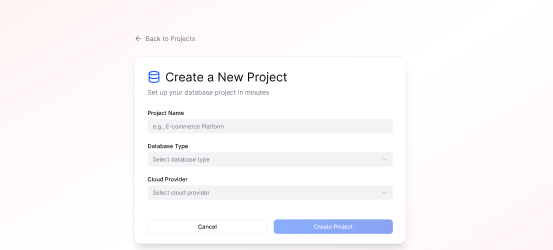
\includegraphics[width=\textwidth]{images/create new project.png}
        \caption{Project Creation Modal}
    \end{subfigure}
    \vspace{5pt}
    \caption{Project management and cloud provisioning interfaces.}
\end{figure}

% --- 3. Display & Filtering ---
\subsubsection*{Advanced Filtering \& Theme Support}
Supports dynamic resource tracking with provider-based filtering and optimization for both Light and Dark modes.

\begin{figure}[H]
    \centering
    \begin{subfigure}[b]{0.48\textwidth}
        \centering
        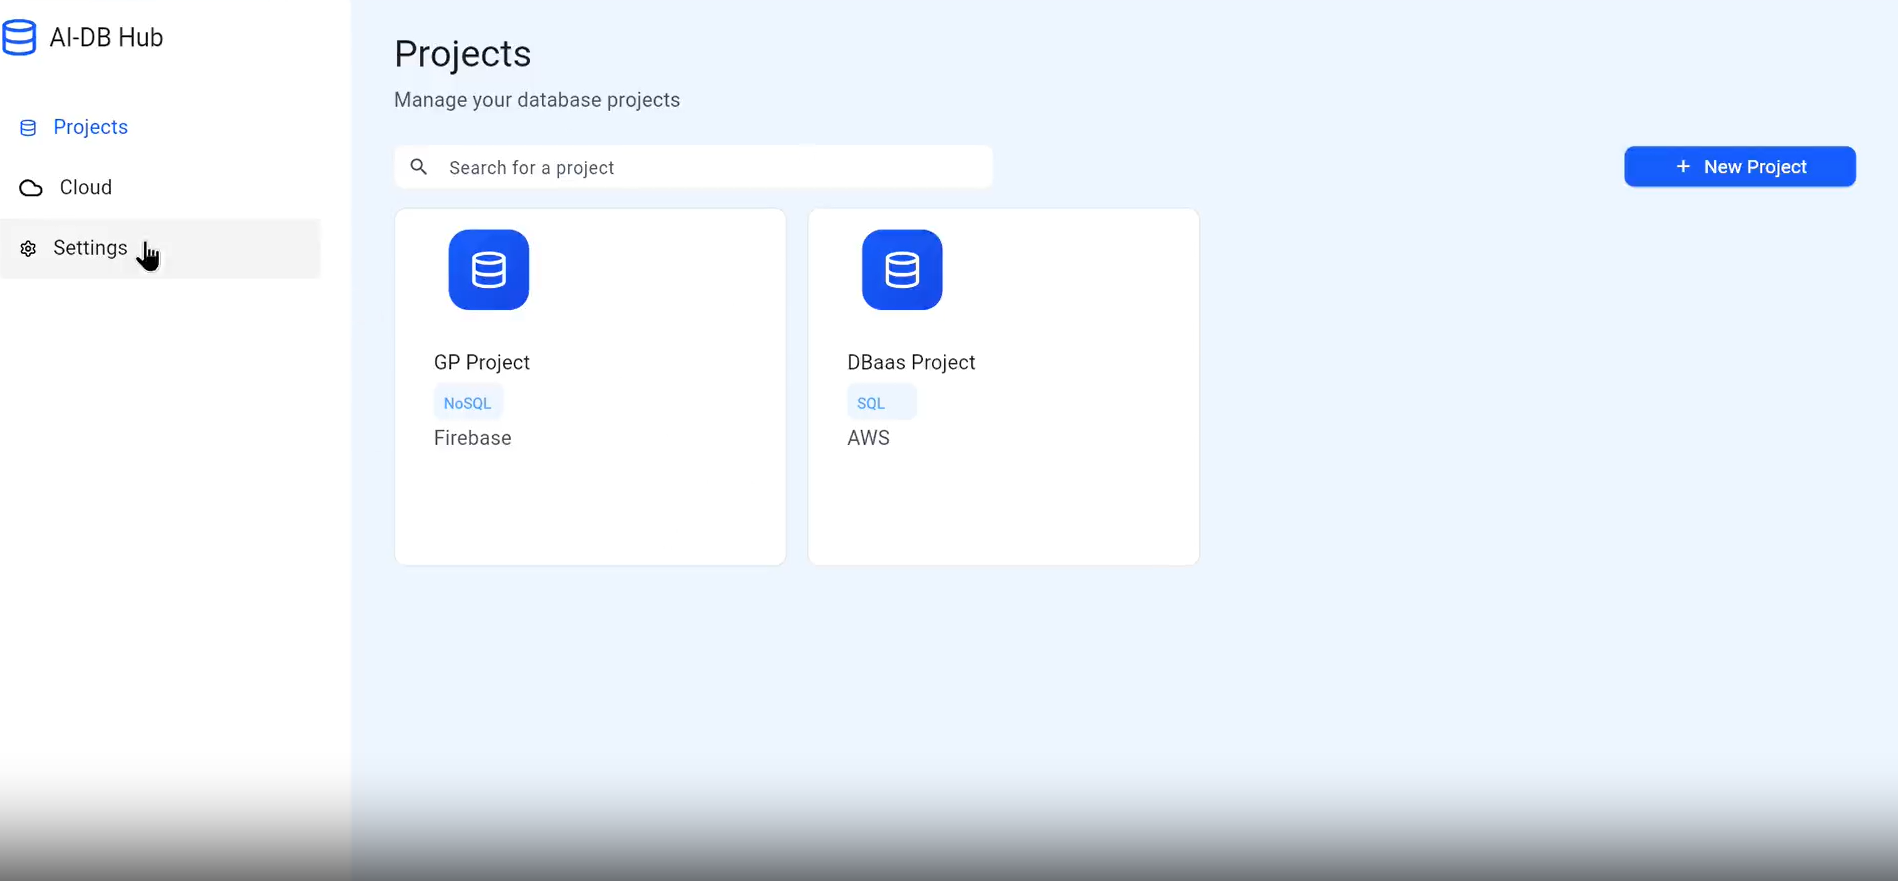
\includegraphics[width=\textwidth]{images/Display exist ploject light.png}
        \caption{Light Mode View}
    \end{subfigure}
    \hfill
    \begin{subfigure}[b]{0.48\textwidth}
        \centering
        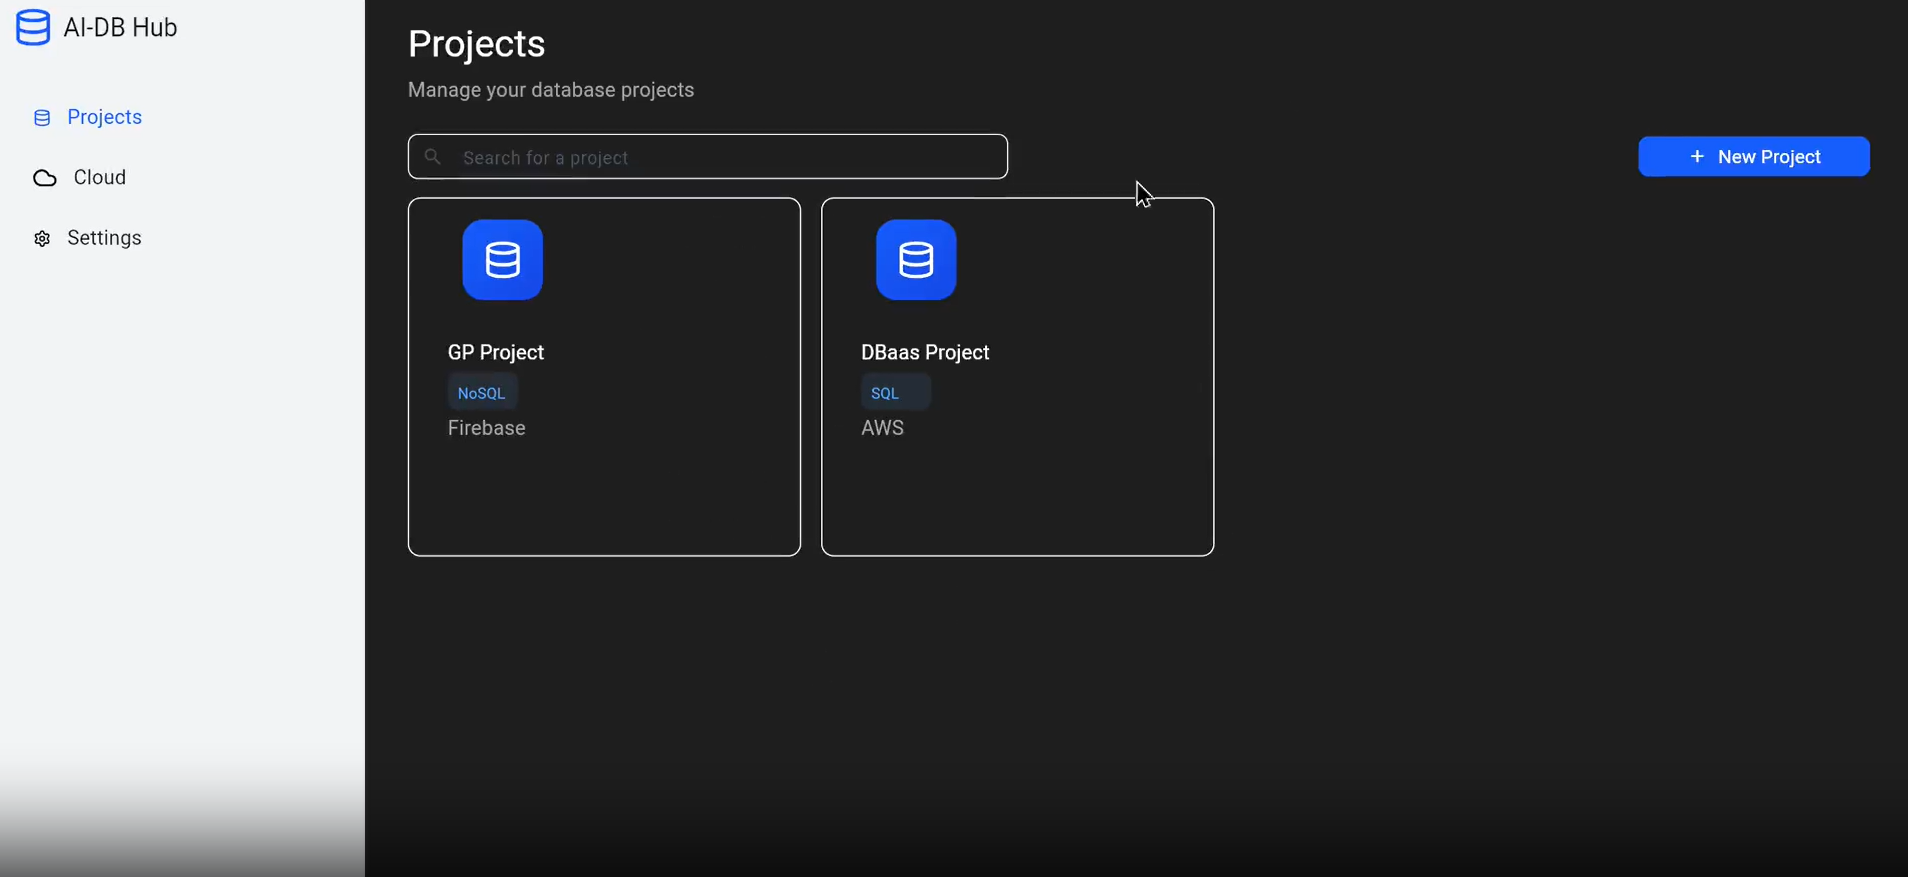
\includegraphics[width=\textwidth]{images/Display exist ploject dark.png}
        \caption{Dark Mode View}
    \end{subfigure}
    \\[10pt] 
    \begin{subfigure}[b]{0.6\textwidth}
        \centering
        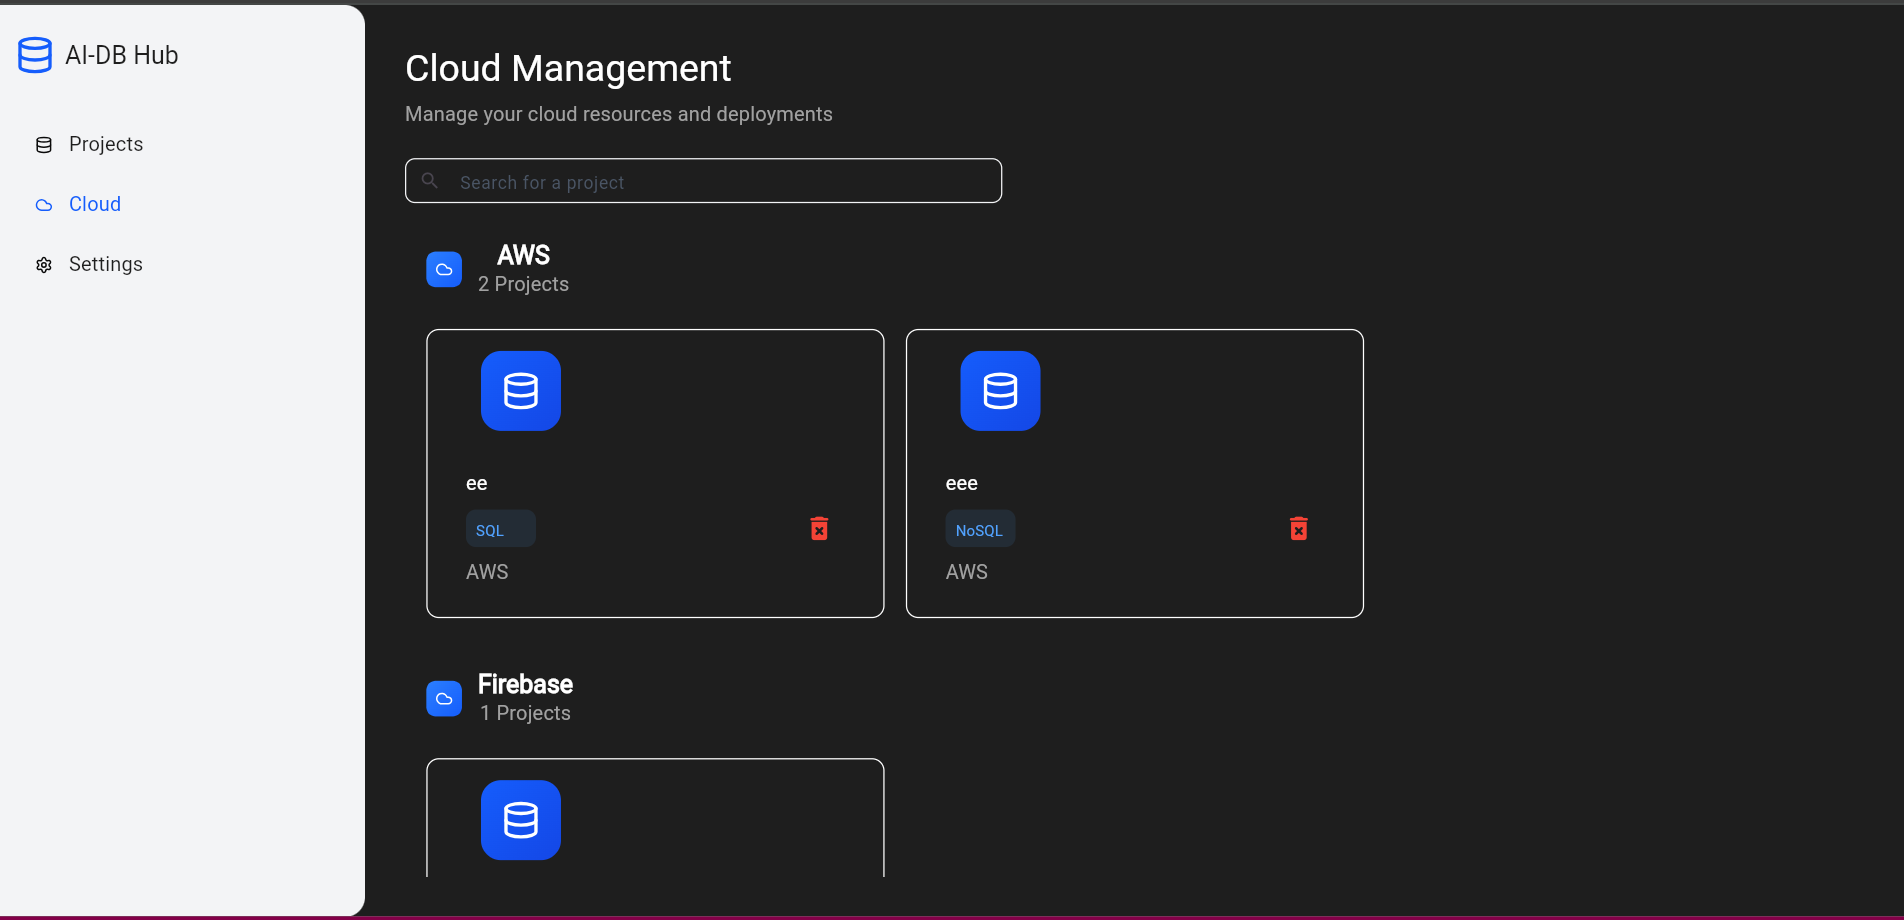
\includegraphics[width=\textwidth]{images/cloud projects filteration.png}
        \caption{Cloud Provider Filtering}
    \end{subfigure}
    \vspace{5pt}
    \caption{Project display with theme toggling and provider filtering.}
\end{figure}



% --- 5. Workspace Sidebars ---
\subsubsection*{Database Workspace Sidebars}
Context-aware navigation for SQL and NoSQL environments, providing access to query editors and schema tools.

\begin{figure}[H]
    \centering
    \begin{subfigure}[b]{0.48\textwidth}
        \centering
        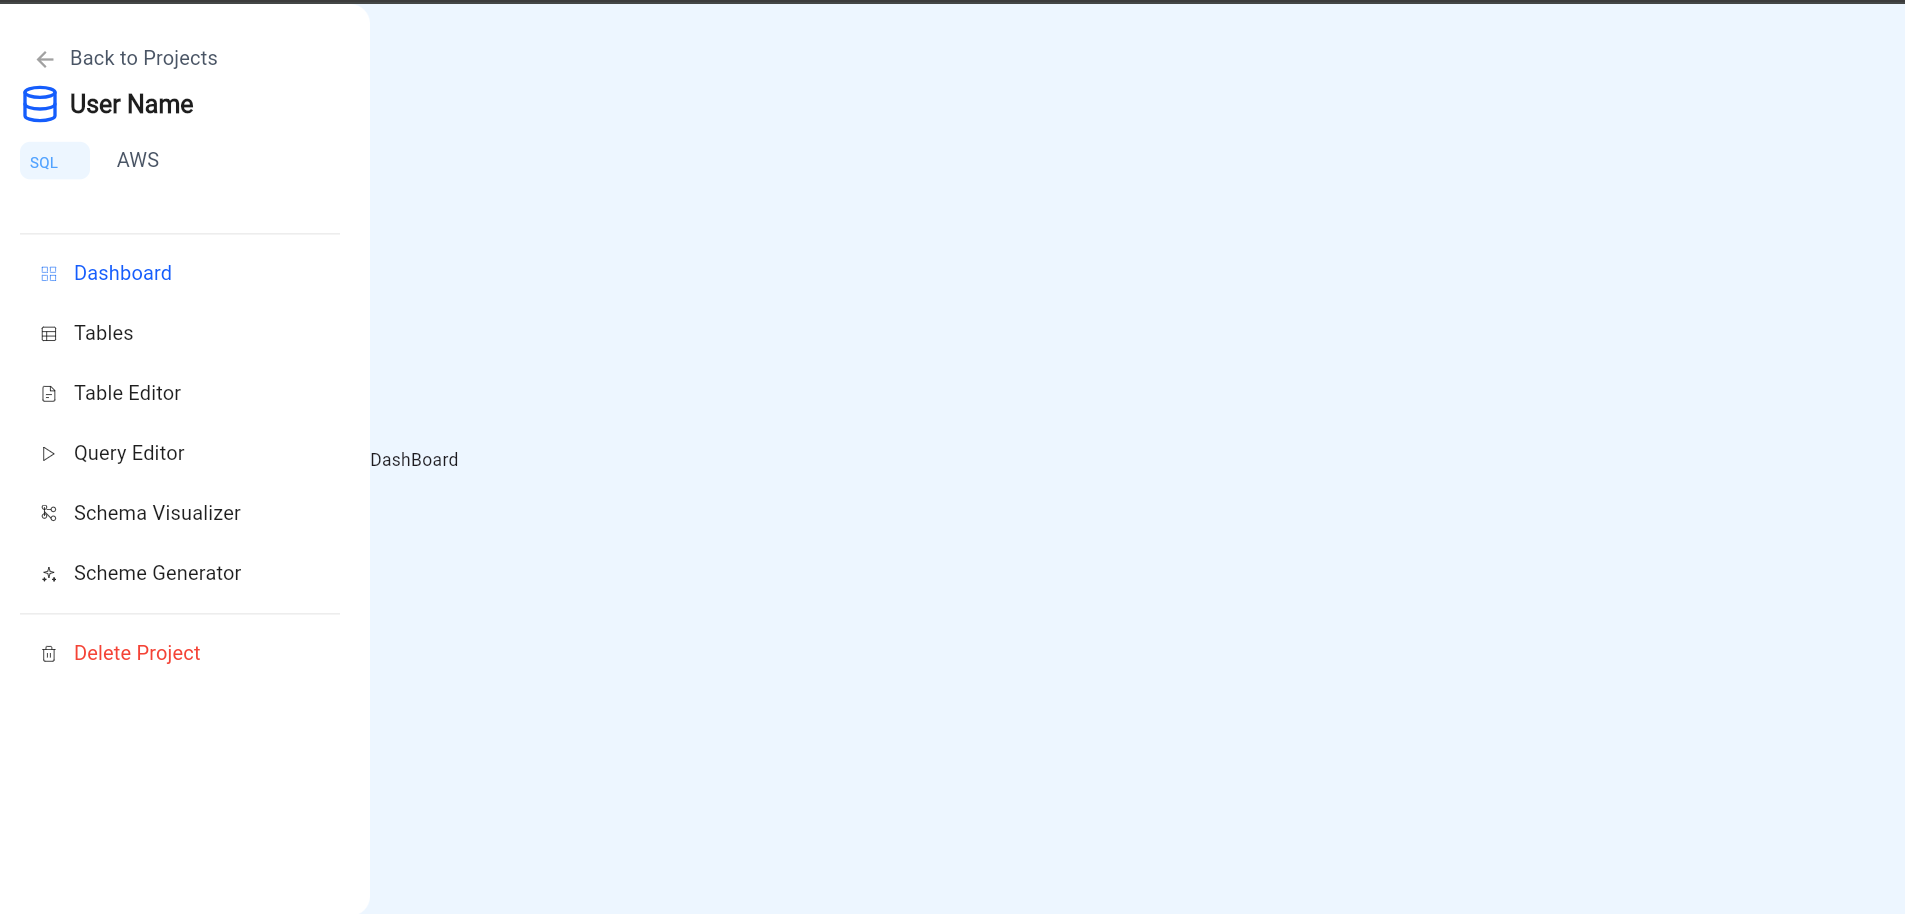
\includegraphics[width=\textwidth]{images/sql tab project.png}
        \caption{SQL Sidebar}
    \end{subfigure}
    \hfill
    \begin{subfigure}[b]{0.48\textwidth}
        \centering
        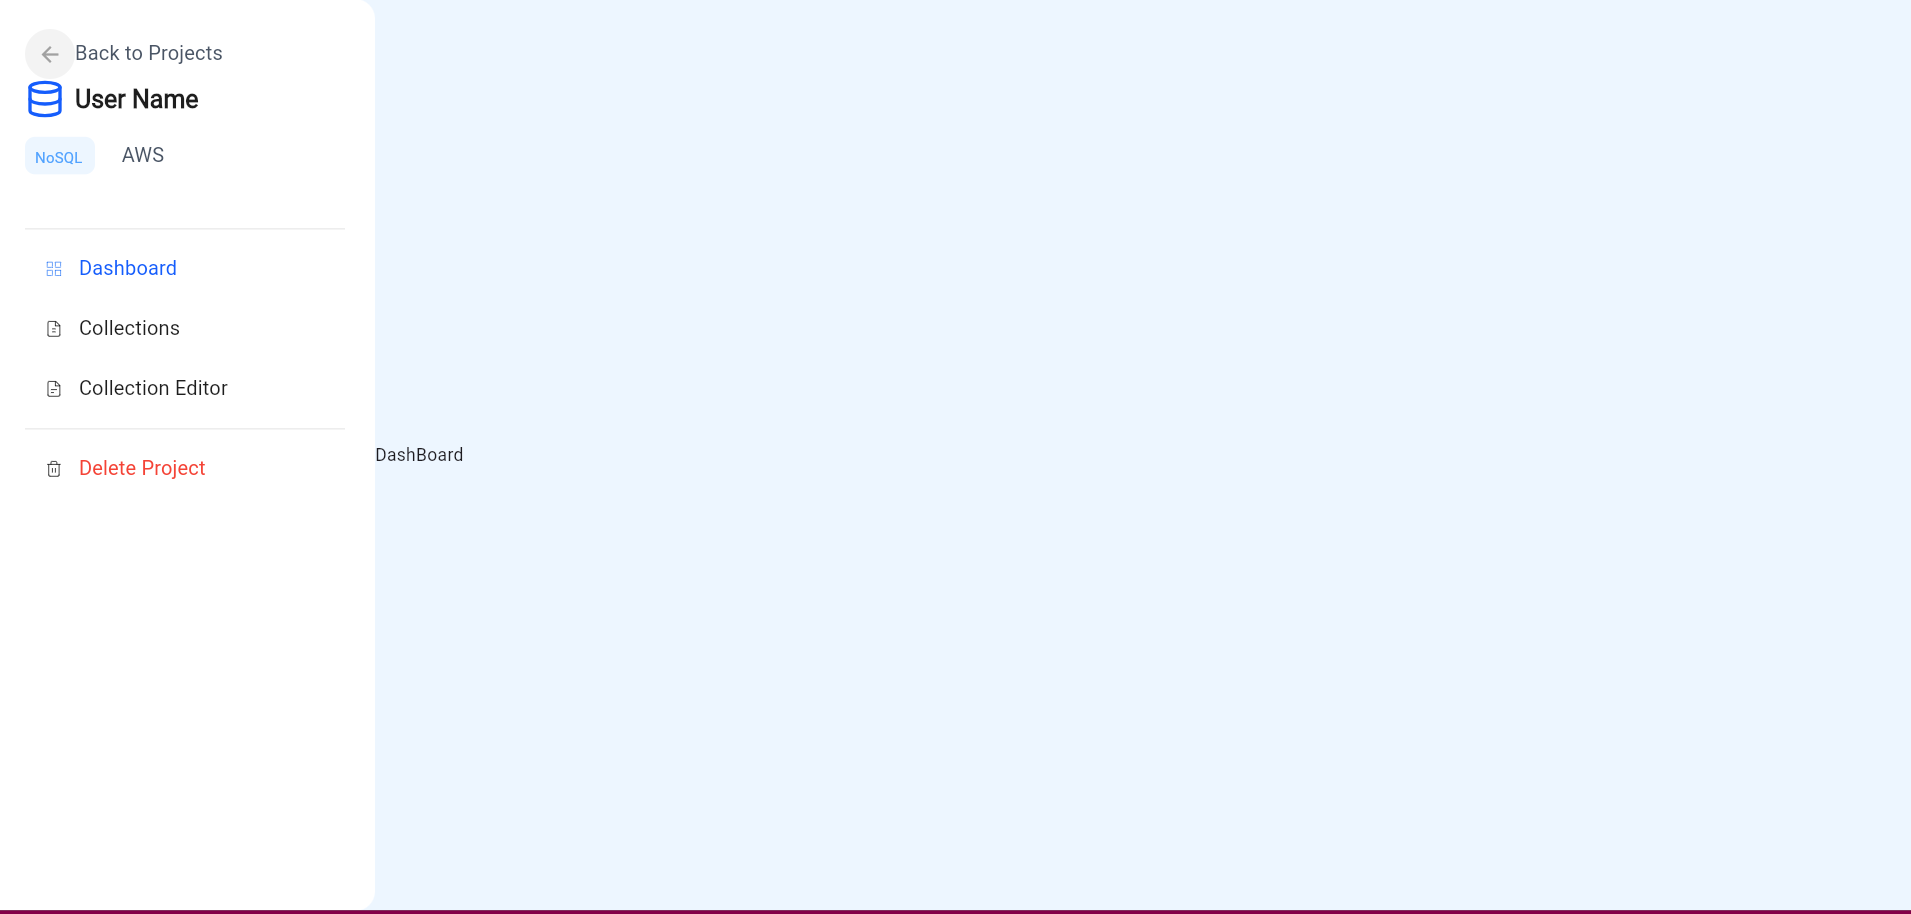
\includegraphics[width=\textwidth]{images/no sql tabs project.png}
        \caption{NoSQL Sidebar}
    \end{subfigure}
    \vspace{5pt}
    \caption{Database workspace sidebars for specialized project management.}
\end{figure}

\subsection{SQL Project Management Tools}

The platform provides a specialized suite of tools dedicated to \textbf{SQL-based projects}. These features are designed to handle relational structures, ensuring data integrity through schema enforcement and providing visual interfaces for complex relational operations.

% --- 1. Empty States (Onboarding) ---
\subsubsection*{Initial Setup and User Guidance}
When a new SQL project is provisioned, the system provides intuitive empty states direct the user to begin by defining their schema or creating their first table.

\begin{figure}[H]
    \centering
    \begin{subfigure}[b]{0.48\textwidth}
        \centering
        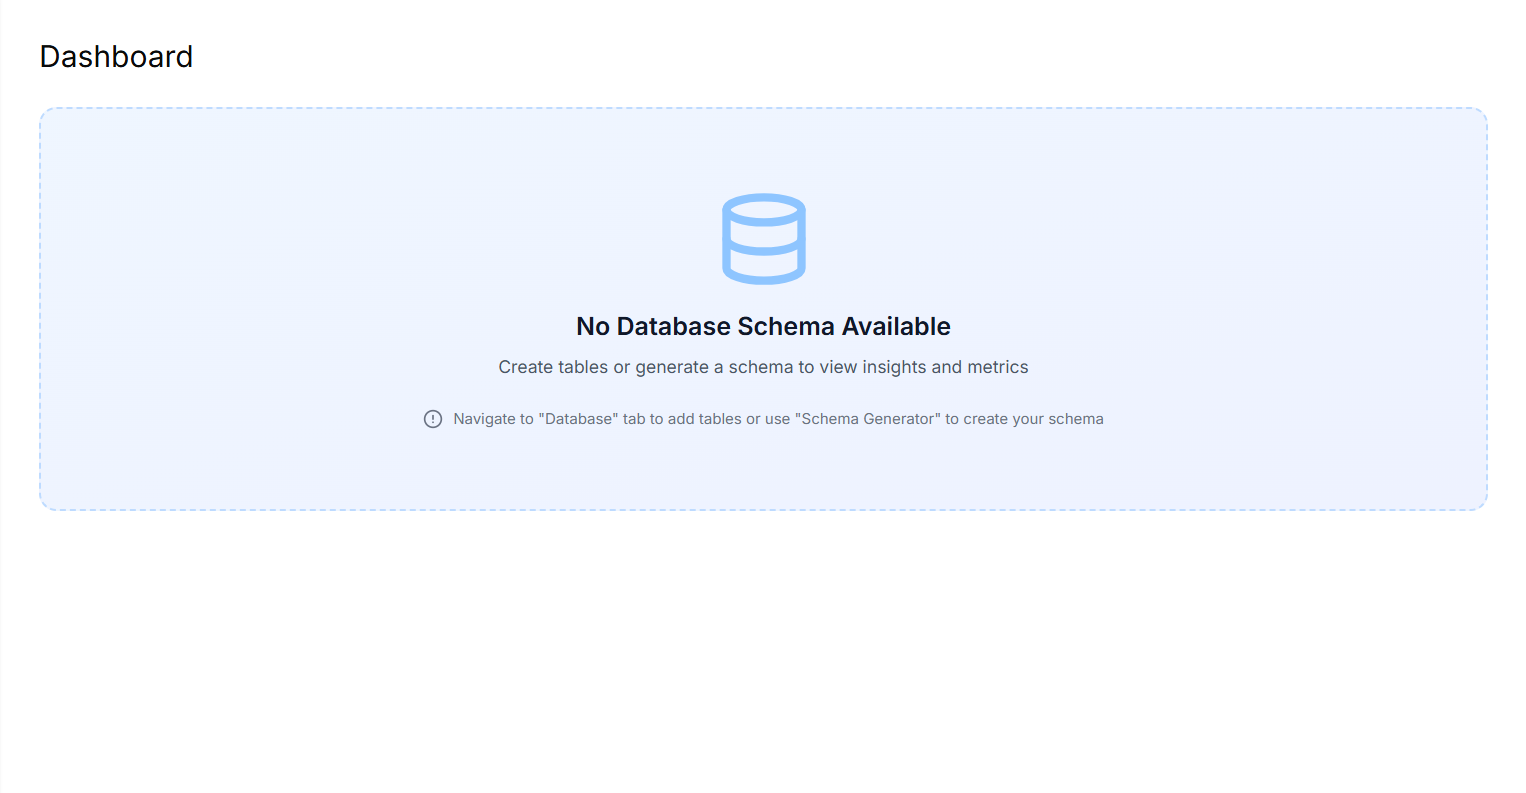
\includegraphics[width=\textwidth]{images/initial_dash_board.png}
        \caption{Initial Dashboard State}
    \end{subfigure}
    \hfill
    \begin{subfigure}[b]{0.48\textwidth}
        \centering
        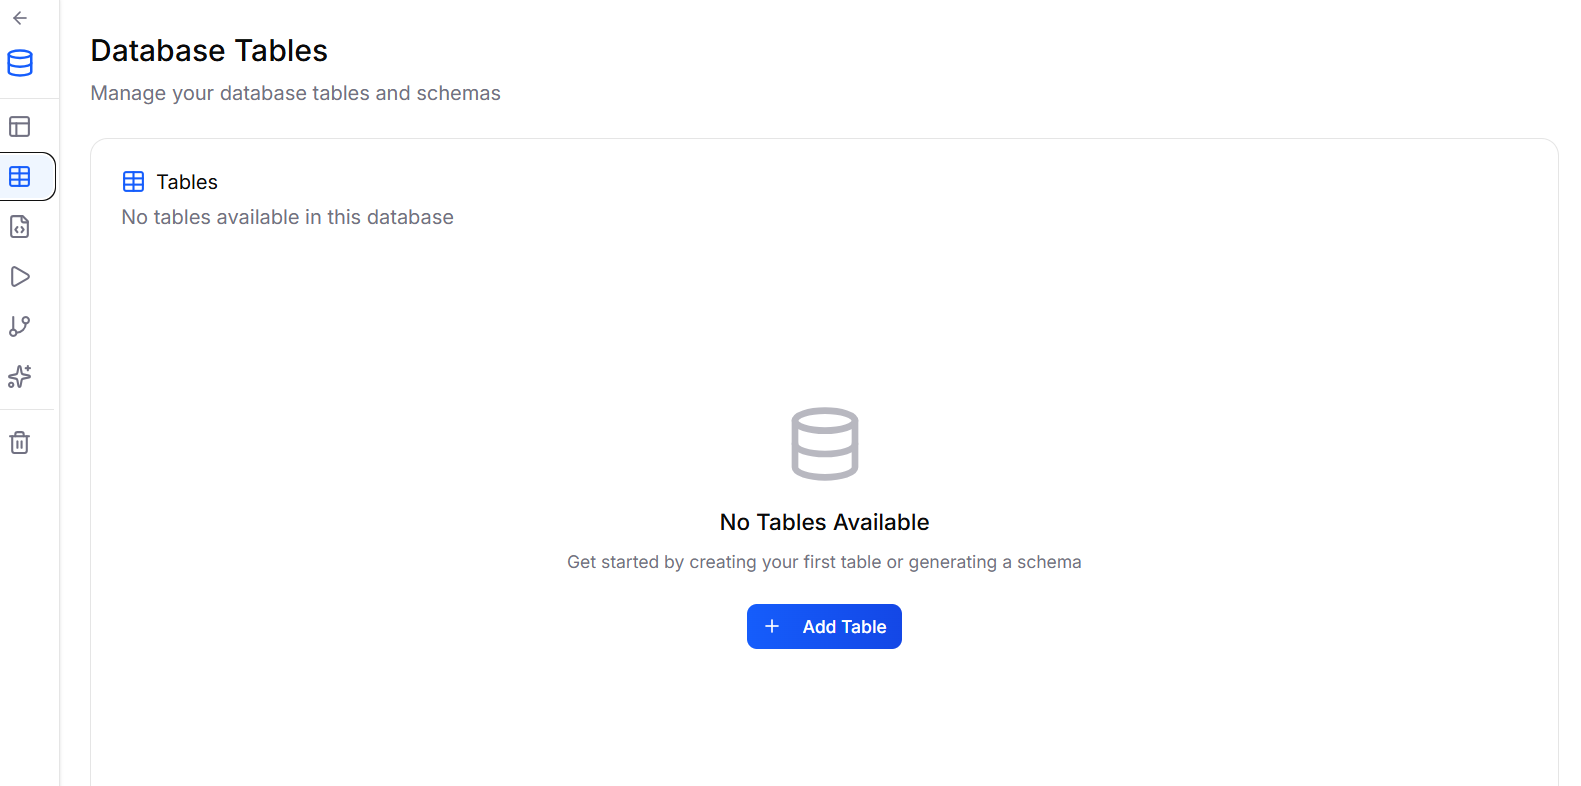
\includegraphics[width=\textwidth]{images/database_tables.png}
        \caption{Empty Tables View}
    \end{subfigure}
    \vspace{5pt}
    \caption{Guided onboarding for newly provisioned SQL databases.}
\end{figure}
\newpage
% --- 2. Table Creation & Operations ---
\subsubsection*{Relational Table Management}
Users can define relational tables through a visual builder. This includes setting primary keys, auto-incrementing sequences (SERIAL), and managing data rows through an interactive grid.

\begin{figure}[H]
    \centering
    \begin{subfigure}[b]{0.48\textwidth}
        \centering
        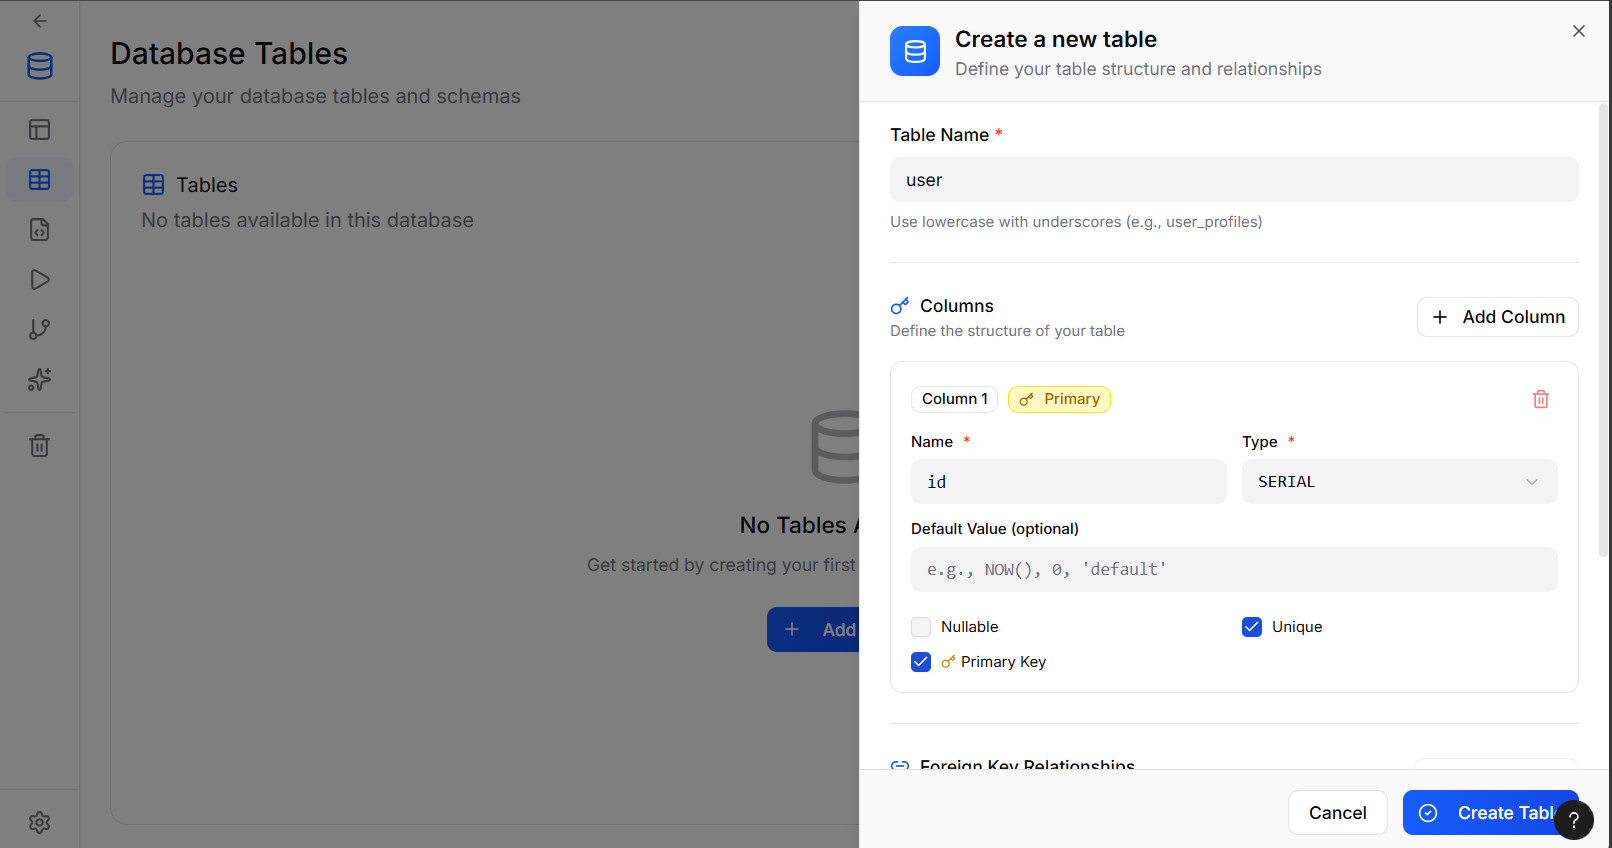
\includegraphics[width=\textwidth]{images/create_tables.png}
        \caption{Creating a new SQL Table}
    \end{subfigure}
    \hfill
    \begin{subfigure}[b]{0.48\textwidth}
        \centering
        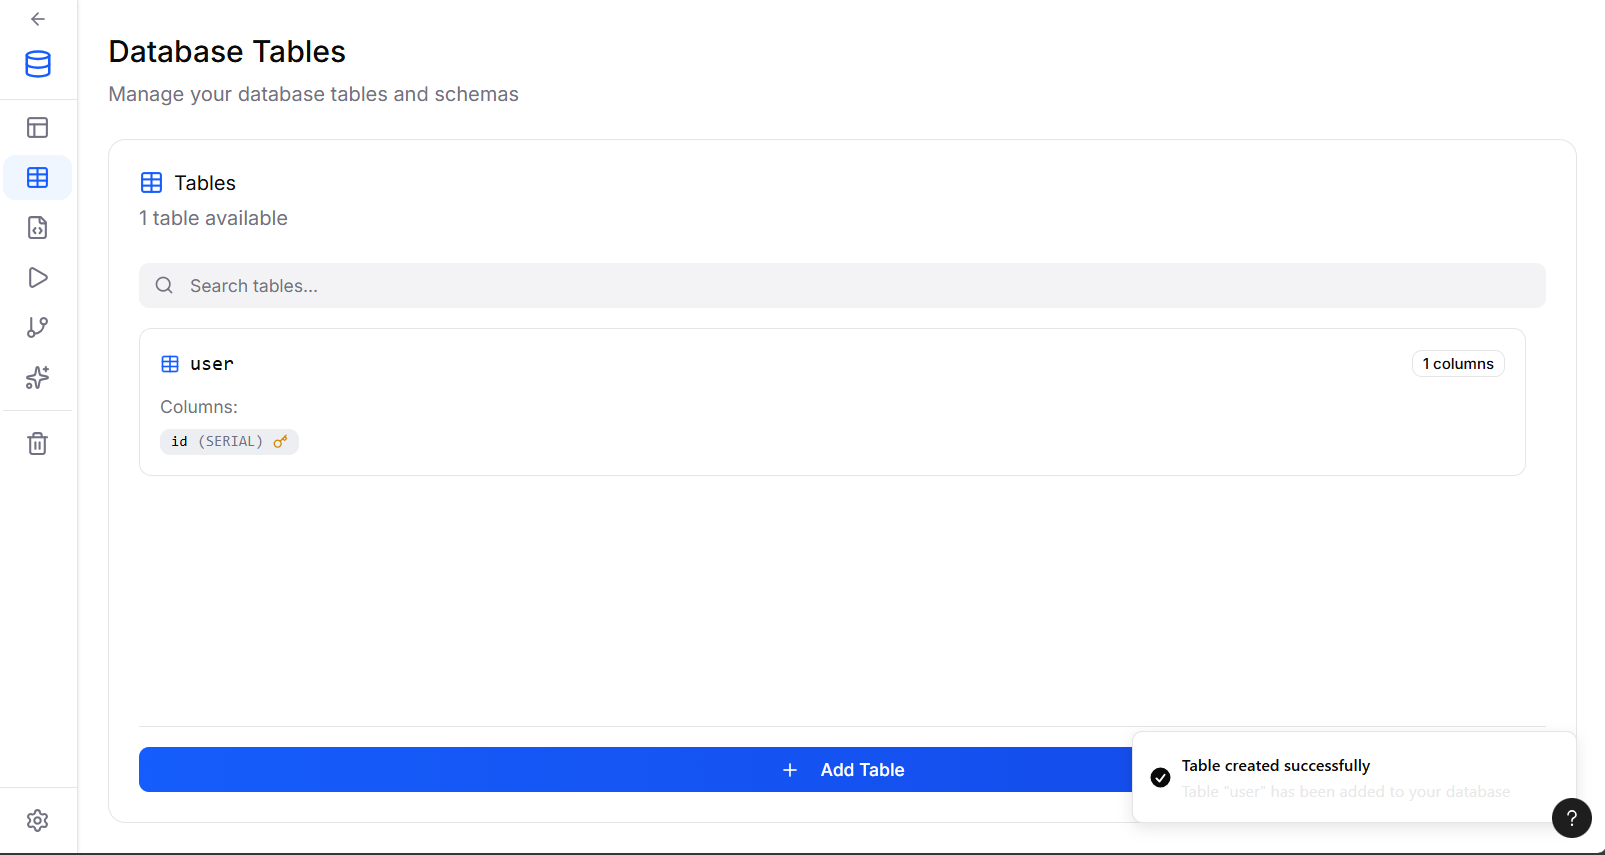
\includegraphics[width=\textwidth]{images/table_created.png}
        \caption{Table Schema Overview}
    \end{subfigure}
    \\[10pt] 
    \begin{subfigure}[b]{0.48\textwidth}
        \centering
        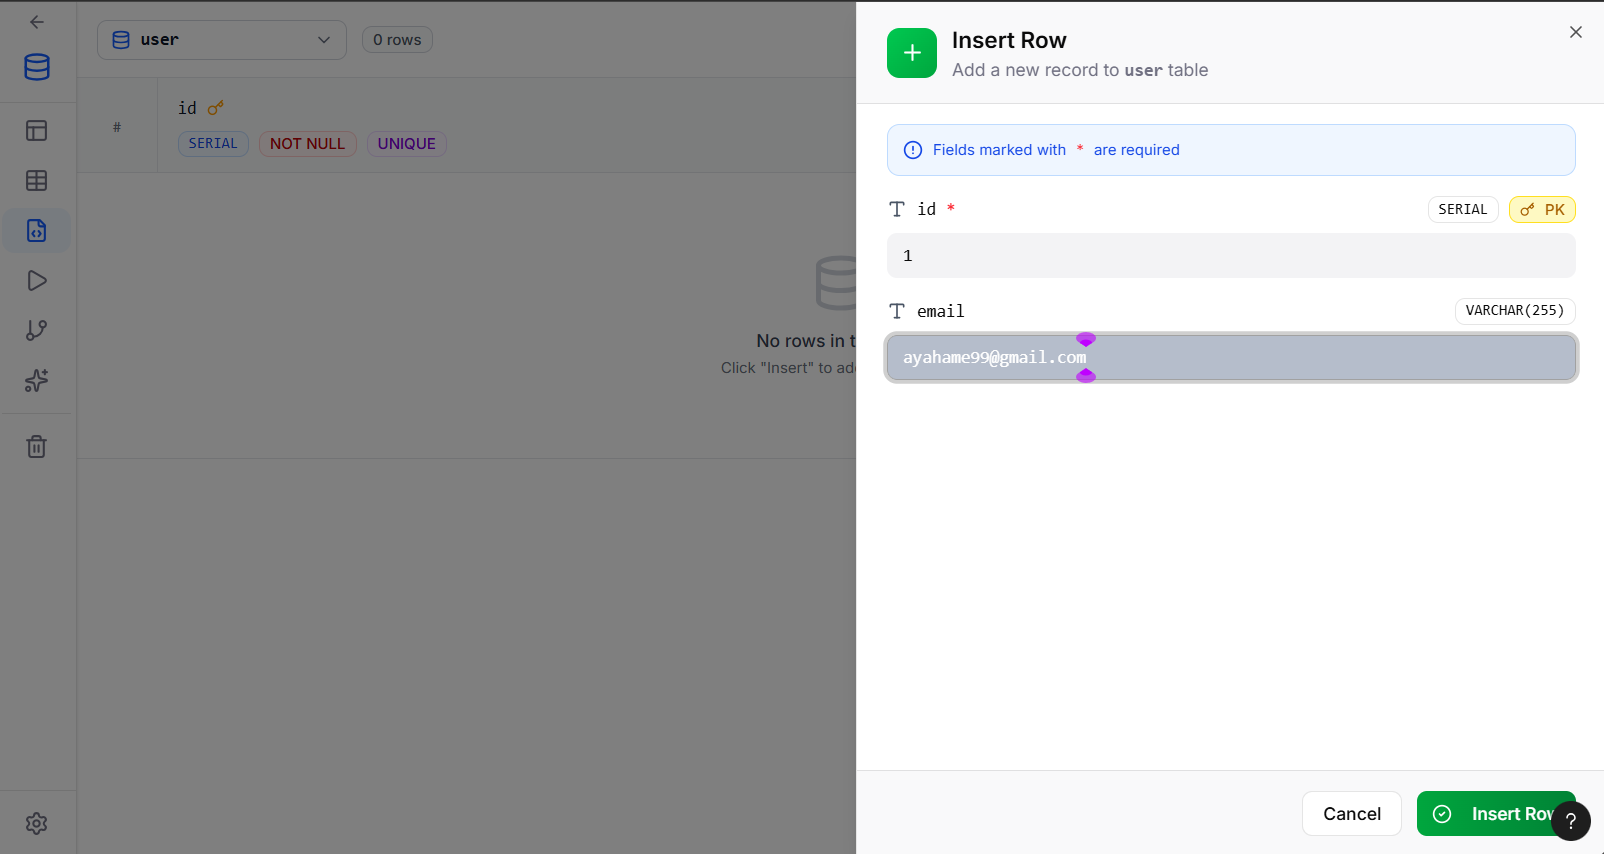
\includegraphics[width=\textwidth]{images/adding_row.png}
        \caption{Data Insertion Interface}
    \end{subfigure}
    \hfill
    \begin{subfigure}[b]{0.48\textwidth}
        \centering
        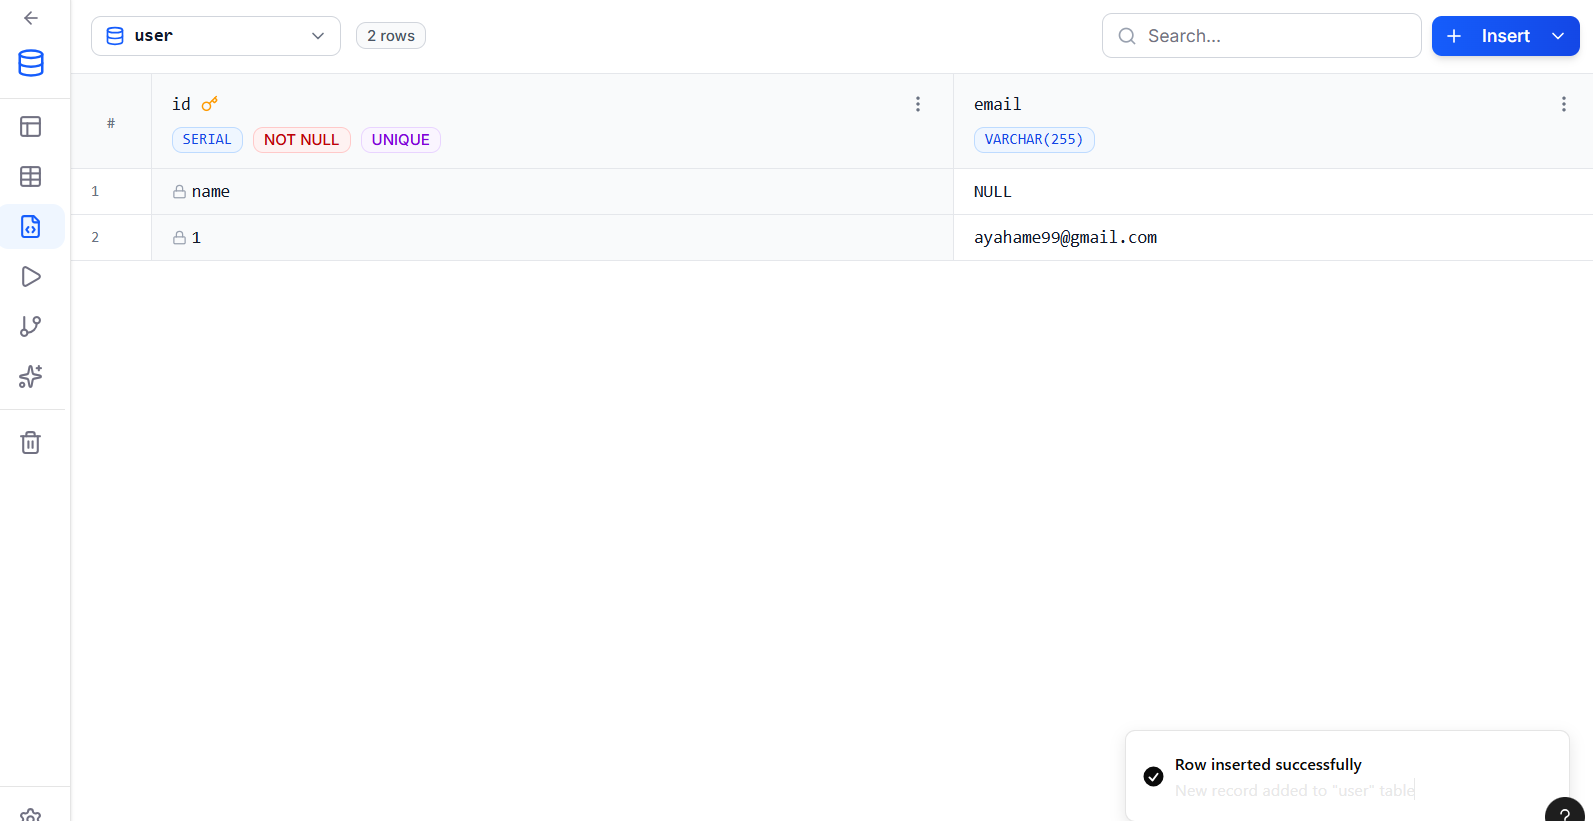
\includegraphics[width=\textwidth]{images/reflect_on_adding.png}
        \caption{Populated Data Grid}
    \end{subfigure}
    \vspace{5pt}
    \caption{Visual workflow for managing SQL tables and records.}
\end{figure}

% --- 3. Schema Evolution ---
\subsubsection*{Schema Evolution and Column Modification}
To support evolving requirements, the platform allows users to alter table structures dynamically, such as adding new columns with specific constraints and data types like VARCHAR.

\begin{figure}[H]
    \centering
    \begin{subfigure}[b]{0.48\textwidth}
        \centering
        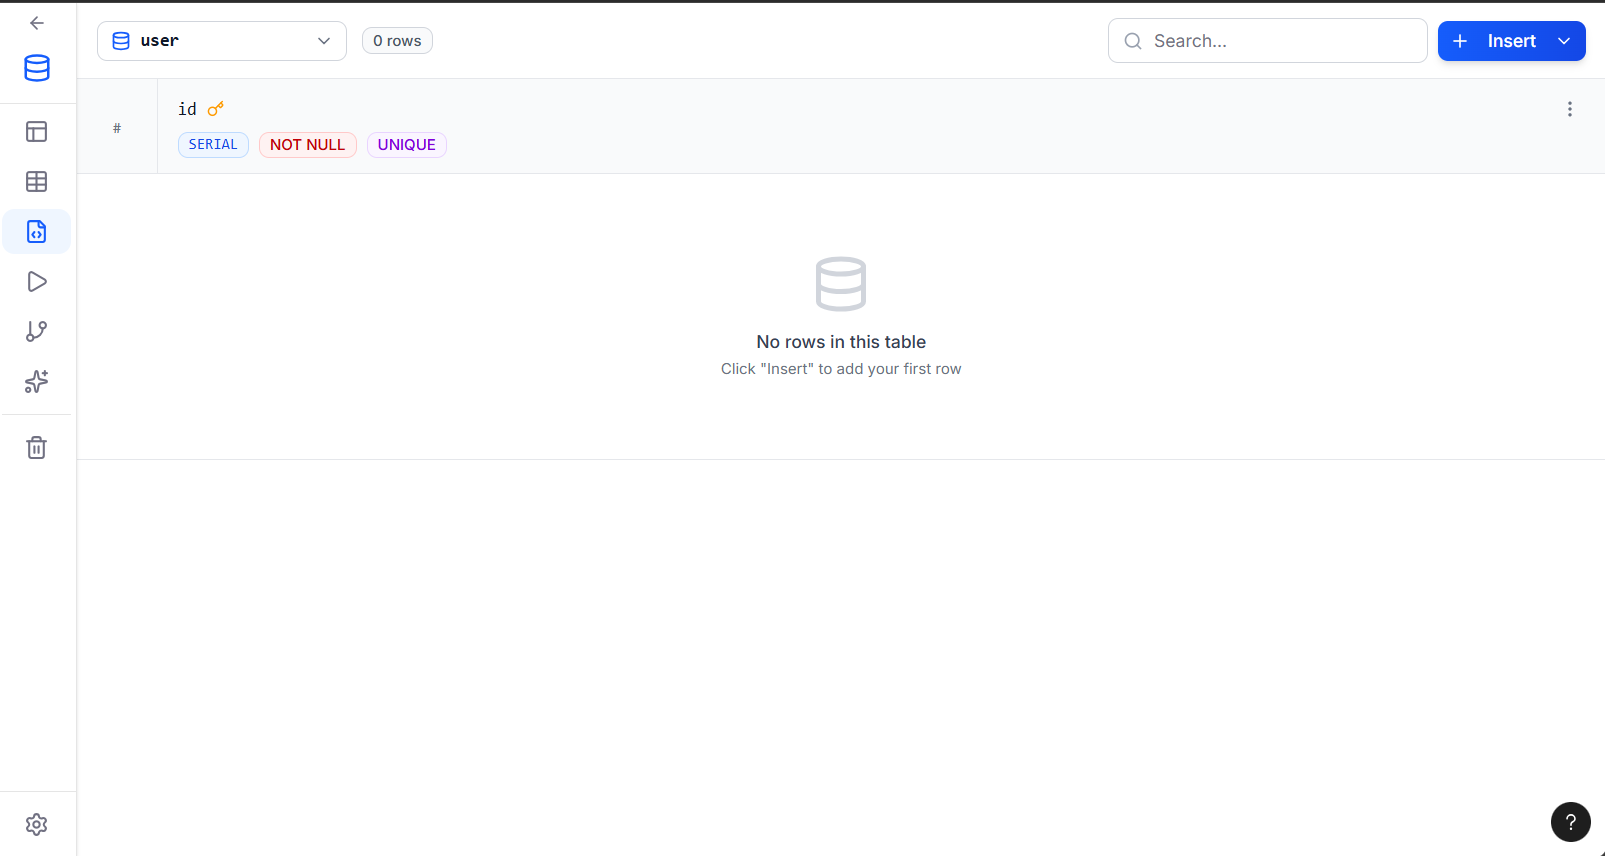
\includegraphics[width=\textwidth]{images/edit_table.png}
        \caption{Structural Edit Mode}
    \end{subfigure}
    \hfill
    \begin{subfigure}[b]{0.48\textwidth}
        \centering
        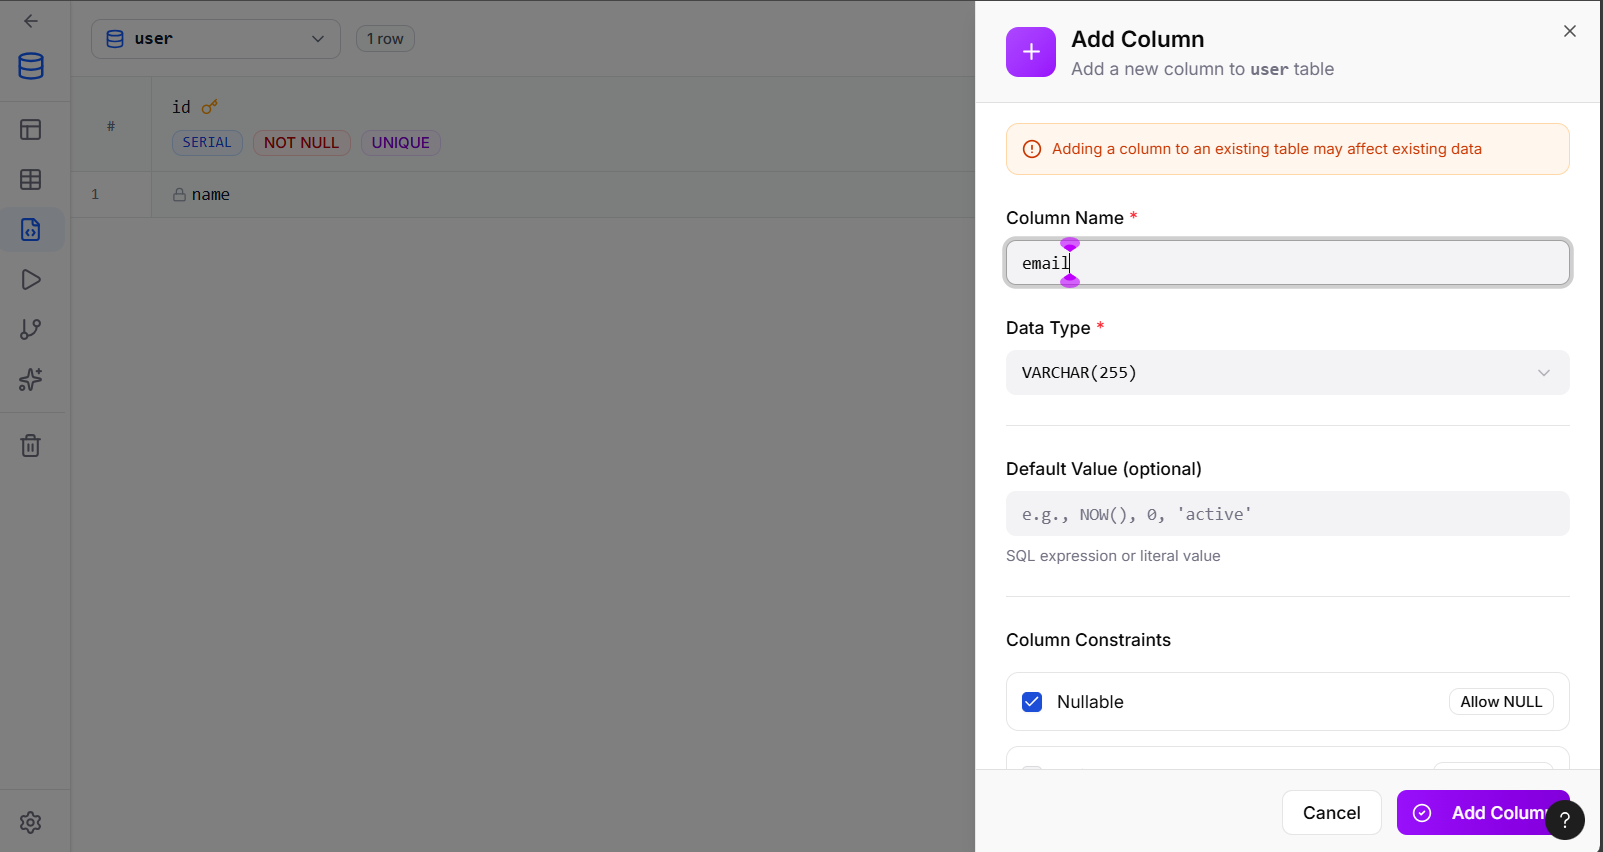
\includegraphics[width=\textwidth]{images/adding column.png}
        \caption{Adding New Columns}
    \end{subfigure}
    \vspace{5pt}
    \caption{Interfaces for modifying existing relational schemas.}
\end{figure}

% --- 4. Querying and Visualization ---
\subsubsection*{SQL Workbench and Schema Visualization}
For advanced users, a full SQL editor to execute different queries on created schemas.

\begin{figure}[H]
    \centering
    \begin{subfigure}[b]{0.45\textwidth}
        \centering
        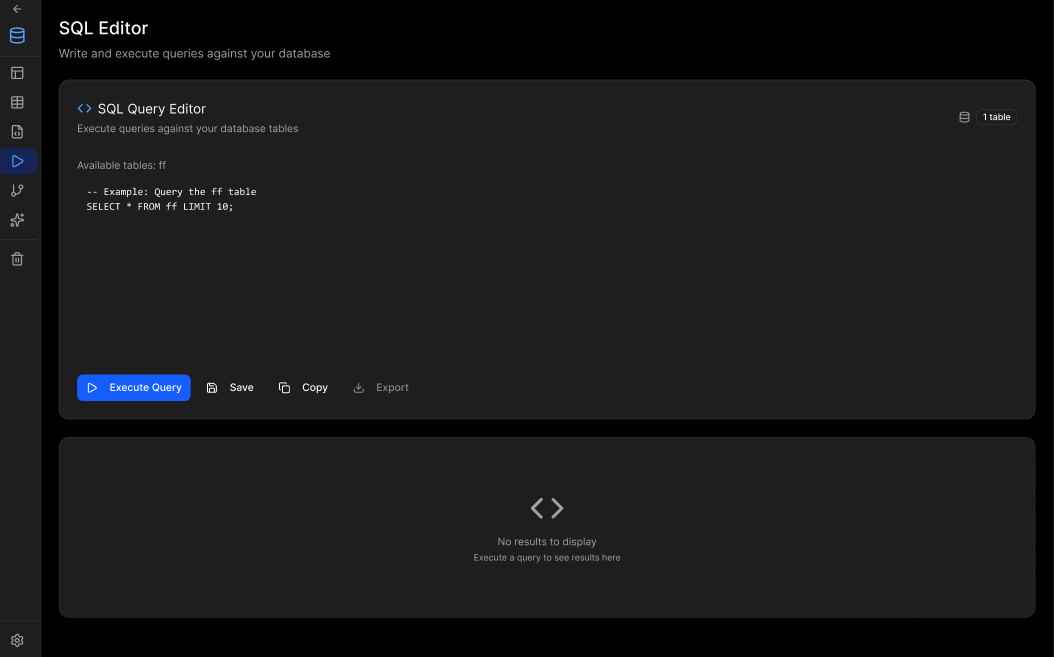
\includegraphics[width=\textwidth]{images/query_dark.png}
        \caption{Dark-themed SQL Editor}
    \end{subfigure}
    \hfill
    \begin{subfigure}[b]{0.53\textwidth}
        \centering
        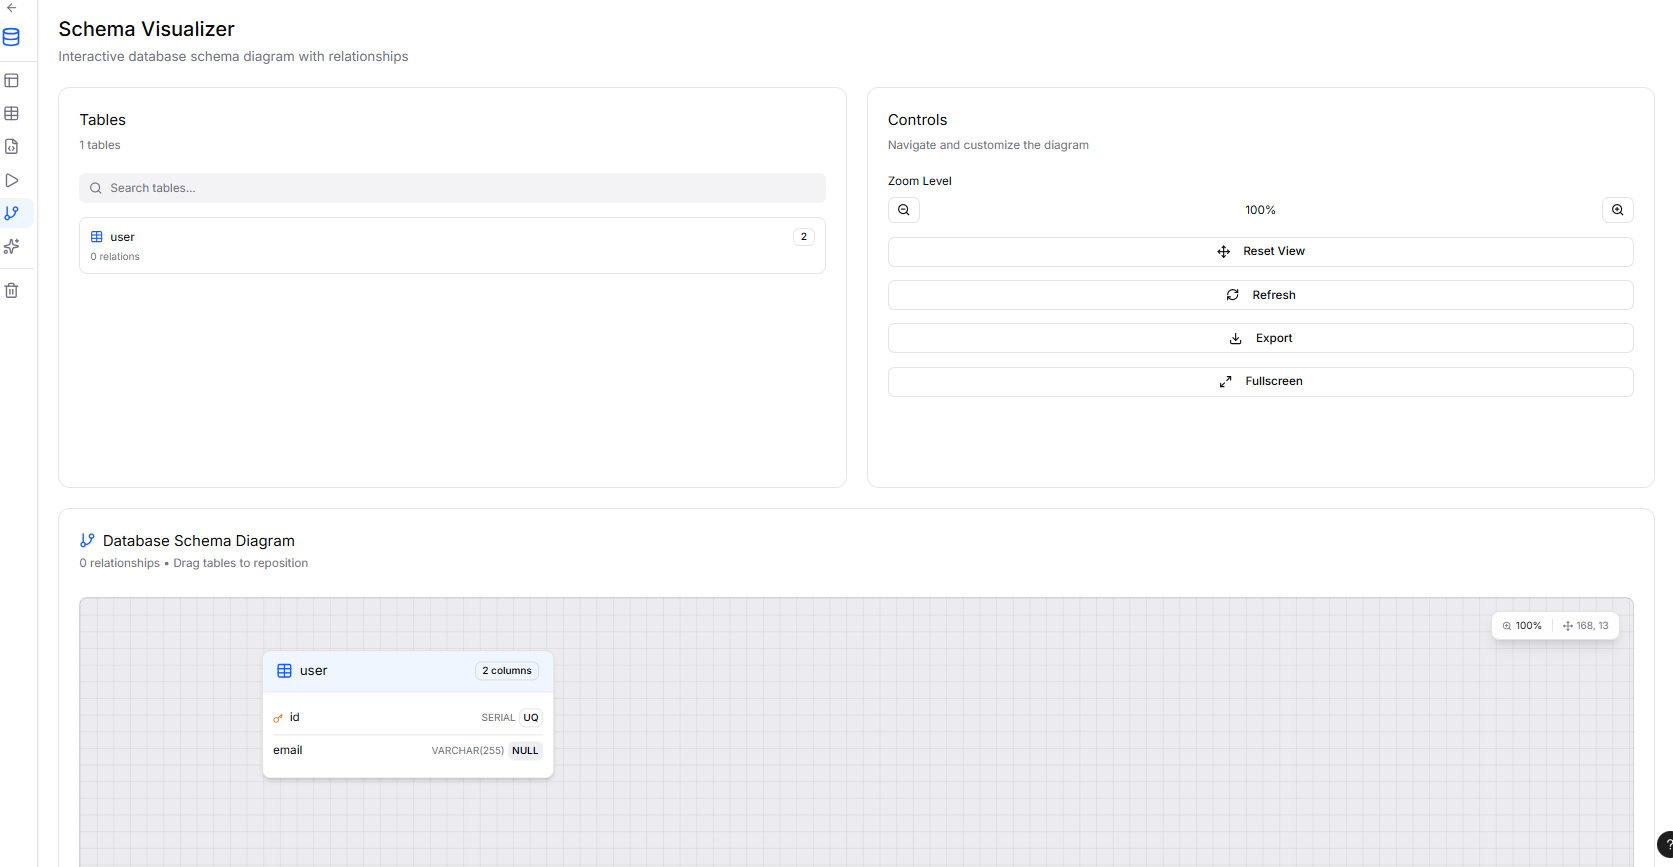
\includegraphics[width=\textwidth]{images/schema_viz.png}
        \caption{Interactive Schema Diagram}
    \end{subfigure}
    \vspace{5pt}
    \caption{Advanced querying and architectural visualization tools.}
\end{figure}
\newpage
% --- 5. Full Settings ---
\subsubsection*{Comprehensive System Settings}
Beyond database operations, the platform includes a full settings dashboard where users can manage their account, UI themes, and global system preferences.

\begin{figure}[H]
    \centering
    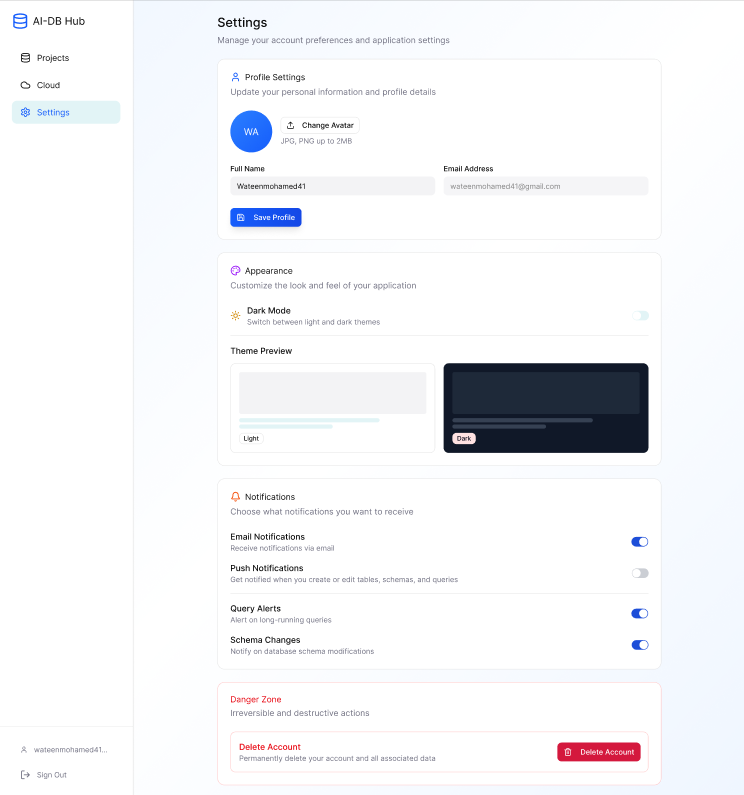
\includegraphics[width=0.9\textwidth]{images/settings_full_screen.png}
    \caption{System-wide settings and personalization interface.}
\end{figure}